\documentclass[a4paper,10pt]{scrartcl}
\usepackage[margin=2cm,bindingoffset=0cm]{geometry}
\usepackage{ucs}
\usepackage[utf8x]{inputenc}
\usepackage[ngerman]{babel}
\usepackage{fontenc}
%\usepackage[pdftex]{graphicx}
\usepackage{listings}
\usepackage{amssymb}
\usepackage{amsmath}
\usepackage{wasysym}
\usepackage{graphicx}
\usepackage[pdftex]{hyperref}
\author{Verena Käfer (2551188), Niklas Schnelle (2573250), Peter Vollmer (2553704)}
\date{erstellt am 15.11.2010\\
Version: 1.0}
\title{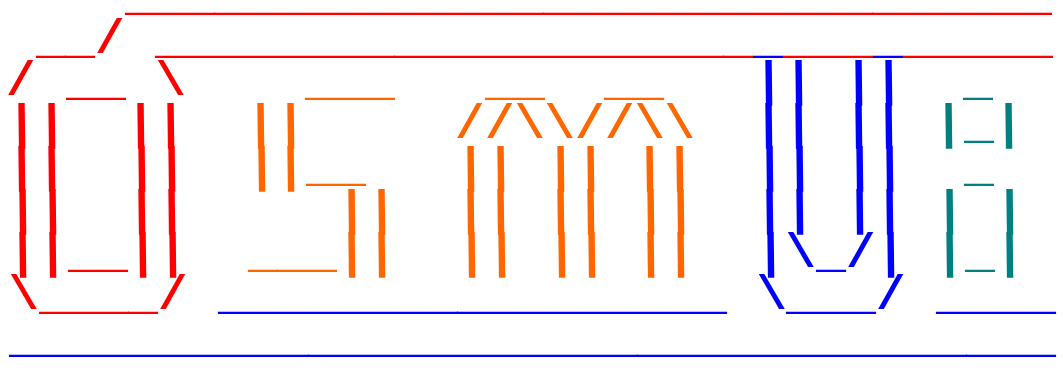
\includegraphics[width=15cm]{../projektplan/Logo_Osmui.png} \\ 
Spezifikation von OsmUi}

\begin{document}
\maketitle
\newpage
\tableofcontents
\newpage

\section{Einleitung}
\subsection{Zweck der Spezifikation}
Bei der Spezifikation handelt es sich um das zentrale Projektdokument. Sie ist Basis aller weiteren Dokumente und
Bezugspunkt in Funktionalitätsfragen. Sie ist daher unbedingt aktuell und konsistent zu halten.\\
Die Spezifikation beschreibt die Funktionen und Anforderungen an das Produkt OsmUi und das zugehörige Projekt.
\subsection{Leserkreis}
Diese Spezifikation richtet sich an:
\begin{itemize}
 \item Die Entwickler von OsmUi
 \item Den Kunden und die Betreuer des SoPra
\end{itemize}

\subsection{Projektüberblick}
In dem Entwicklungsprojekt OsmUi soll eine grafische Benutzeroberfläche für das Kommandozeilenwerkzeug \href{http://wiki.openstreetmap.org/wiki/Osmosis}{Osmosis}
entwickelt werden. Zu diesem Zweck überträgt OsmUi das abstrakte Pipelinekonzept von Osmosis auf eine grafische Darstellung, welche die gesamte Funktionalität von Osmosis zugänglich macht, dabei aber deutlich benutzerfreundlicher sein soll.\\
Während bei Osmosis ein langer Kommandozeilenaufruf eine Pipeline zur Verarbeitung von OpenStreetMap Daten beschreibt, wobei sich der Benutzer die Befehle merken
und korrekt in der gewünschten Reihenfolge aufschreiben muss, soll es mit OsmUi möglich sein eine Verarbeitungspipeline ``zusammen zu klicken''.\\
Hierbei kann die Funktionsweise der einzelnen Tasks sowie deren Interaktion der Benutzeroberfläche von OsmUi entnommen werden.
%\subsection{Konventionen} %Kommt noch

\section{Akteure}
\subsection{Benutzer}
Bei OsmUi gibt es grundsätzlich nur eine Nutzerklasse. Es wird davon ausgegangen, dass OsmUi benutzt wird um eine Verarbeitungspipeline für OpenStreetMap Daten
zu erstellen, welche anschließend durch Osmosis ``ausgeführt'' wird. Hierbei wird davon ausgegangen, dass der Nutzer grundlegende Kentnisse 
von Datenverarbeitung und OpenStreetMap hat.

\section{Nichtfunktionale Anforderungen}
\subsection{Entwurfseinschränkungen}
\subsubsection{Entwurfskonzept}
OsmUi wird nach dem \href{http://de.wikipedia.org/wiki/KISS-Prinzip}{KISS-Prinzip} entwickelt, d.h. entscheidend für die Qualität der Software soll
sein, wie gut die Hauptfunktionen unterstützt werden. Bessere Hauptfunktionalität ist einem größeren Funktionsumfang unterzuordnen.\\
Im Fall von OsmUi heißt dies, dass das Hauptaugenmerk auf dem einfachen und sinnvollen Erstellen von Verarbeitungspipelines, sowie deren Import und Export liegt.\\
Weniger wichtig sind hingegen ``Luxusfunktionen'' wie direktes Anzeigen des Verarbeitungsergebnisses (was auf Grund der Vielfalt der Funktionen von Osmosis
und der Verarbeitungsdauer ohnehin nicht immer sinnvoll ist) oder das direkte Aufrufen von Osmosis.
\subsubsection{Systemumgebung}
Systemumgebung ist das \textbf{Java Runtime Environment in Version 1.6 und höher (SE)}. Dabei ist OsmUi als reine Java Anwendung zu entwickeln, so dass
keine externen Abhängigkeiten bestehen und OsmUi auf allen Java SE kompatiblen Systemen eingesetzt werden kann.
Eventuell wird intern die Bibliothek \textbf{JGraph} eingesetzt, diese wird dann aber direkt mit ausgeliefert
und ist ebenso in platformunabhängigem Java geschrieben. 
\subsubsection{Layout und Gestaltung}
OsmUi soll ab einer Auflösung von 1024x768 und bis zu einer Systemschriftgröße 24 benutzbar sein. Alle Fenster sollen, wenn dies sinnvoll ist, skalierbar sein und den eventuell gewonnenen Platz
nutzen. Um Benutzer von Multimonitorsystemen und exotischen Windowmanagern zu entlasten soll die Positionierung von neuen Fenstern nativ erfolgen. Es
sollen insbesondere keine Fenster in eine errechnete Bildschirmmitte von OsmUi positioniert werden.
\subsection{Robustheit}
OsmUi soll als Software möglichst robust arbeiten, d.h. unter allen Bedingungen korrekt arbeiten. Dies soll durch defensive Programmierung erreicht werden.
Jedoch sollen Benutzereingaben möglichst früh geprüft werden, so dass tiefere Funktionen den Daten ``vertrauen'' können. Dies sichert zudem ab, dass klar ist, welcher
Programmteil für die Prüfung zuständig ist. Nämlich immer der erste, der die nötigen Informationen hat.\\
Weiterhin wird die Robustheit durch das KISS-Prinzip unterstützt, da weniger Funktionen besser entworfen und getestet werden können.
\subsection{Portabilität}
OsmUi soll durch den Einsatz reinen Javas auf allen Systemen mit Java SE 1.6 Unterstützung lauffähig sein. Als Exportformate für Osmosis Aufrufskripte
werden .bat und .sh (/bin/sh) unterstützt, womit alle Posix Systeme sowie Windows abgedeckt sind.
\subsection{Erweiterbarkeit}
Das Programm muss keine besonderen Erweiterungsfunktionalitäten wie etwa ein Pluginsystem zur Verfügung stellen, jedoch werden der Programmcode und die Systemarchitektur
so gestaltet, dass OsmUi leicht und schnell an neue oder veränderte Osmosis Funktionen angepasst werden kann.
\section{Distributionsform und Installation}
OsmUi wird als ausführbares JAR Archiv ausgeliefert, welches direkt ausgeführt werden kann.


\section{Funktionale Anforderungen}
\subsection{Mengengerüst}
Bei OsmUi handelt es sich um eine Einzelplatzanwendung und es wird keine Netzwerkfunktion genutzt, somit gibt es zu jedem Zeitpunkt genau einen Nutzer.\\
Beim Erstellen/Laden/Speichern von Verarbeitungspipelines muss OsmUi in der Lage sein, mit Pipelines von bis zu 100 Tasks zuverlässig zu arbeiten -
eine künstliche Beschränkung nach oben besteht jedoch nicht.
\subsection{Laden und Speichern von Verarbeitungspiplines als Osmosis Aufrufscript}
Dem KISS-Prinzip folgend bietet OsmUi eine einheitliche Laden- und Speichern-Funktion, die sowohl bereits vorhandene Osmosis Aufrufscripts als auch durch OsmUi
selbst erstellte Verarbeitungspiplines, laden kann. Die Speicherung erfolgt als Osmosis Aufrufskripte.\\
Dies ermöglicht auch beim Wechsel des Werkzeugs einen leichten Zugriff auf alle mit OsmUi erstellten Dateien.
\subsubsection{Laden}
Eine der Hauptfunktionen von OsmUi stellt das Laden von Aufrufscripten dar. Dabei können sowohl Dateien im .bat - als auch im .sh Format (mit \#!/bin/sh Shebang),
sowie Textdateien, in denen nur eine Osmosis Parameterliste steht, geladen werden. Sie werden direkt im Pipelinebearbeitungsfeld angezeigt und
stehen zur Bearbeitung bereit.
\subsubsection{Speichern}
Zum Speichern wählt der Benutzer entweder eine neue Datei aus, die, wenn vorhanden, überschrieben und sonst neu erstellt wird. Oder er überschreibt die gerade bearbeitete Datei.
Der Dateityp kann hierbei zwischen .sh Script und .bat gewählt werden.


\subsection{Benutzeroberfläche}
Die Benutzeroberfläche von OsmUi ist in zwei Teile aufgeteilt: die Taskauswahlbox und die Pipelinebox. Desweiteren gibt es ein Anwendungsmenü und beim Bearbeiten eines Tasks
wird es ein weiteres Einstellungsfenster geben.\\
\begin{center}
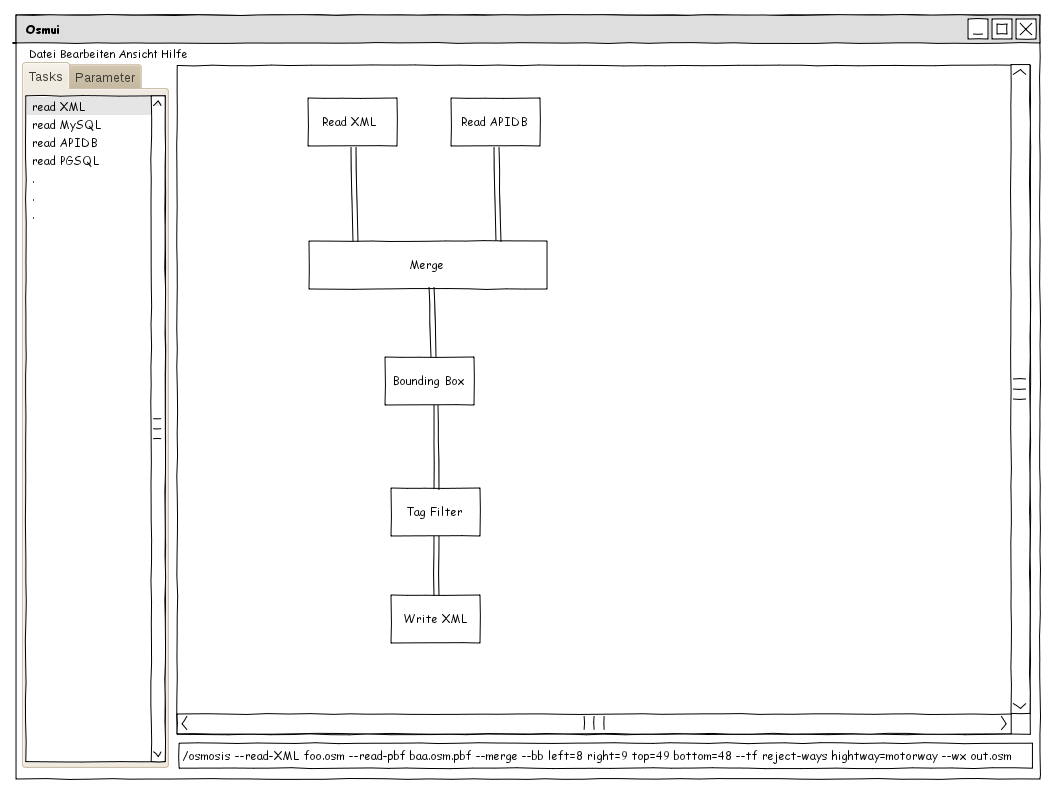
\includegraphics[width=15cm]{ui_prototype/OsmUi_Startseite.png}
\end{center}
\subsubsection{Taskauswahlbox}
Im linken Teil der Benutzeroberfläche wird eine Liste der gerade zum Einfügen verfügbaren Tasks dargestellt. Dabei kann die Darstellung als Icon,
Text oder Kombination erfolgen. Es werden nur Tasks angezeigt die gerade auch einfügbar sind. \\
Am Anfang sind dies zum Beispiel alle Tasks, (z.B. read XML) die keinen Streameingang haben. Ist in der Pipelinebox ein Task ausgewählt, so
sind nur diejenigen Tasks sichtbar, die mit dem/den Ausgang/Ausgängen des ausgewählten Task kompatibel sind.\\
So wird verhindert, dass der Benutzer Pipelines bauen kann, die nicht durch Osmosis ausführbar sind.
\subsubsection{Pipelinebox}
In der Pipelinebox wird die Pipeline grafisch dargestellt und es können Tasks zum Bearbeiten ausgewählt werden. Ist ein Task ausgewählt so können seine Eigenschaften
bearbeitet oder ein neuer Task über die Taskauswahlbox - wie oben beschrieben - angefügt werden. Desweiteren kann eine Verbindung zu einem anderen Task, der noch offene
Inputs hat, hergestellt werden.
\subsubsection{Taskeinstellungsdialog}
Wählt der Benutzer einen Task aus, so stellt OsmUi einen Dialog zur Verfügung, in dem alle - für den jeweiligen Tasktyp vorhandenen - Parameter eingegeben werden können.
Hierbei kann die Eingabe eingeschränkt sein: als Spanne von Zahlen, als Kartenausschnitt oder als freier Text erfolgen. Dabei wird der für
den Datentyp beste Eingabemodus gewählt.\\
\begin{center}
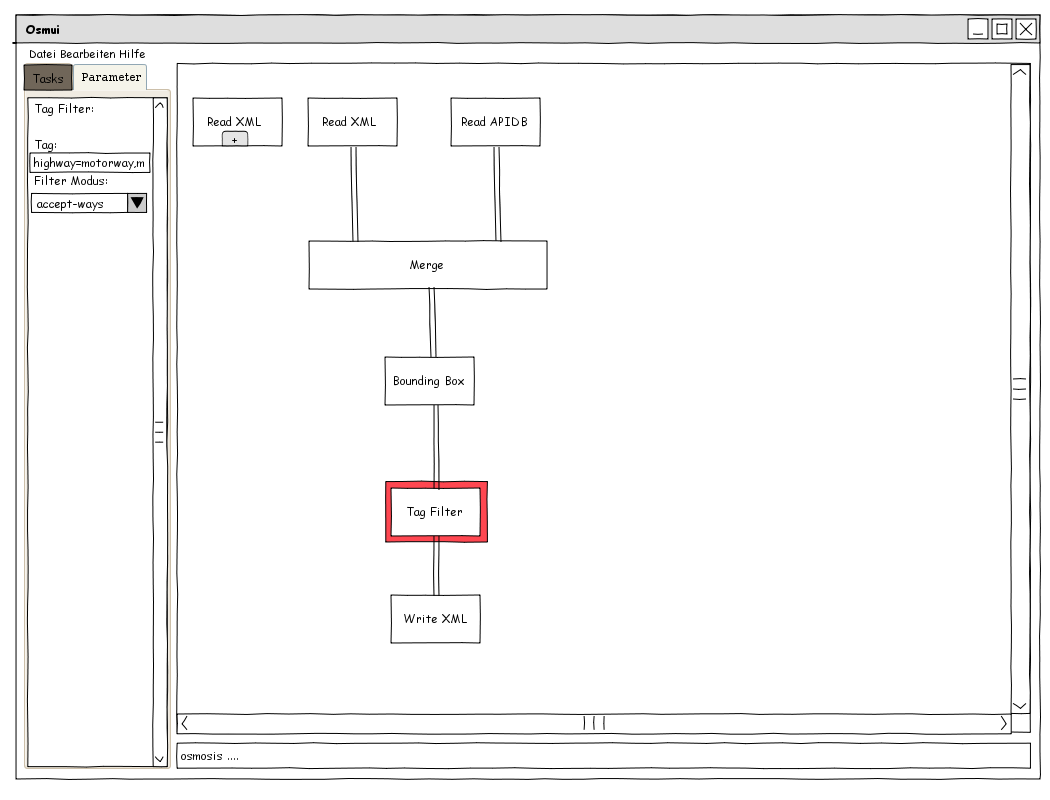
\includegraphics[width=15cm]{ui_prototype/OsmUi_Parameter_Optionen.png}
\end{center}
\subsubsection{Kopierleiste}
Um die aktuell dargestellte Pipeline direkt kopieren zu können, wird sie als Osmosis-Aufruf unter der Pipelinebox angezeigt.
\begin{center}
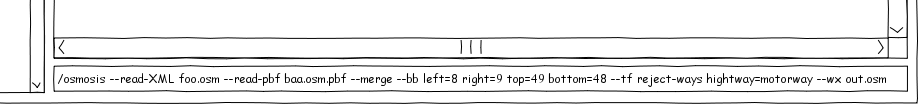
\includegraphics[width=15cm]{ui_prototype/OsmUi_Leisteklein.png}
\end{center}

\subsubsection{Menüleiste}
\begin{itemize}
\item Datei\\
Beim Klicken auf den Menüeintrag \textbf{Datei} öffnet sich ein Dialog. Der Benutzer kann zwischen \textbf{Neu} (Öffnen einer neuen Pipeline), \textbf{Laden...} (Laden einer gespeicherten Datei), \textbf{Speichern} (automatisches speichern der aktuellen Pipeline), \textbf{speichern unter} (speichern der vorhandenen Datei an einem selbst gewählten Ort) und \textbf{schließen} (das Programm wird geschlossen) wählen. 
\\ 
\begin{center}
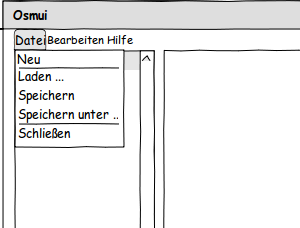
\includegraphics[width=7cm]{ui_prototype/OsmUi_Dateiklein.png}
\end{center}
\item Bearbeiten\\
Beim Klicken auf den Menüeintrag \textbf{Bearbeiten} öffnet sich ein Dialog. Der Benutzer kann zwischen \textbf{Rückgängig} (die letzte Änderung wird wieder rückgängig gemacht) und \textbf{wiederherstellen} (eine rückgängig gemachte Änderung wird wieder hergestellt) wählen.
\\
\begin{center}
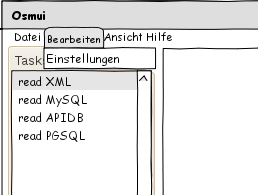
\includegraphics[width=7cm]{ui_prototype/OsmUi_Bearbeitenklein.png}
\end{center}
\item Hilfe\\
Beim Klicken auf den Menüeintrag \textbf{Hilfe} öffnet sich ein Dialog. Der Benutzer kann zwischen \textbf{Hilfe} (Onlinehilfe wird geöffnet) und \textbf{Über...} (Informationen zu OsmUi werden geöffnet) entscheiden.
\\
\begin{center}
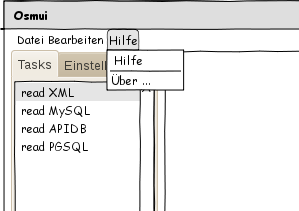
\includegraphics[width=7cm]{ui_prototype/OsmUi_Hilfeklein.png}
\end{center}
\end{itemize}

\subsubsection{Lokalisation}
OsmUi wird eine übersetzte Benutzeroberfläche für mindestens die Sprachen Deutsch und Englisch bieten. Dabei wird die aktuell verwendete
Sprache aus den hierfür vorgesehenen Umgebungsvariablen eingelesen, um sie ohne Interaktion durch den Benutzer in dessen System einzugliedern.
\newpage
\section{Use Cases}
\subsection{Diagramm}
\begin{center}
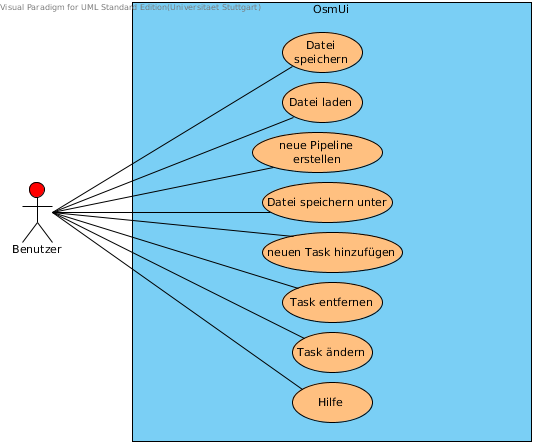
\includegraphics[width=15cm]{Use-Cases.png}
\end{center}
\subsection{Beschreibungen}
\begin{center}
\ \\
\begin{tabular}{|p{5cm}|p{10cm}|}
\hline Name & \textbf{Datei laden} \\ 
\hline Ziel & gespeicherte Daten in OsmUi anzuzeigen \\ 
\hline Vorbedingung & Eine gespeicherte Datei ist vorhanden \\
\hline Nachbedingung & Die Datei wurde geladen und \\ 
\hline Nachbedingung im Sonderfall & Sonderfall OsmUi hat keine Daten geladen und zeigt Zustand vor dem Ladeversuch \\ 
\hline Akteure & Benutzer \\ 
\hline Normalablauf & 1 Der Benutzer klickt auf Datei.
\newline 
2 OsmUi zeigt den Menüeintrag Datei
\newline
3 Der Benutzer klickt auf Datei laden.
\newline
4 OsmUi zeigt die Dateiauswahlroutine.
\newline 
5 Der Benutzer wählt die gewünschte Datei aus
\newline
6 Der Benutzer bestätigt dies mit Klick auf Button ''Öffnen''.
\newline
7 OsmUi lädt die Datei und zeigt sie in der Piplinebox an.
\\ 
\hline Sonderfall 5a) & 5a.1 Der Benutzer klickt auf ''Abrechen''
\newline
5a.2 OsmUi lädt keine Daten und zeigt den vorherigen Zustand.\\
\hline Sonderfall 6a) & 6a.1 Der Benutzer klickt aber auf ''Abrechen''
\newline
6a.2 Osmui lädt keine Daten und zeigt den vorherigen Zustand.\\
\hline Sonderfall 7a) & Pipelinebox ist nicht leer.
\newline 
7a.1 Osmui lädt die Datei in die Piplinebox einer neuen Instanz von OsmUi.\\
\hline Sonderfall 7b)& Datei ist zwischenzeitlich nicht mehr verfügbar.
\newline
 7b.1 OsmUi versucht Datei zu lesen bricht dann ab und zeigt einen entsprechenden Fehlerdialog an.
\newline
 7b.2 Benutzer klickt auf Button ''Ok''.
\newline
$ \rightarrow$ Schritt 4
\\
\hline Sonderfall 7c)& Benutzer besitzt keine Leserechte zur ausgewählten Datei.
\newline
$ \rightarrow$ Schritt 7b.1 
\\
\hline Sonderfall 7d)& Dateityp wird nicht unterstützt.
\newline
$ \rightarrow$ Schritt 7b.1 
\\
\hline 
\end{tabular} 
\vspace{0.7cm}
\\
\begin{tabular}{|p{5cm}|p{10cm}|}
\hline Name & \textbf{Datei speichern} \\ 
\hline Ziel & Aktuelle Datei soll gespeichert werden \\ 
\hline Vorbedingung & Die aktuelle Datei wurde schon einmal gespeichert \\ 
\hline Nachbedingung & Die Datei wurde gespeichert \\ 
\hline Nachbedingung im Sonderfall 1) & Die Datei wurde neu gespeichert \\ 
\hline Nachbedingung im Sonderfall 2) & Die Datei wurde nicht gespeichert\\
\hline Akteur & Benutzer \\ 
\hline Normalablauf & - Der Benutzer klickt den Speicher-Button 
\newline
- Die Datei wird gespeichert
\\
\hline Sonderfall 1) & - Der Benutzer klickt auf den Speicher-Button, aber die Datei ist vorher nicht gespeichert worden
\newline
- Das Speichern-unter-Menü öffnet sich
\newline
- weiter wie im Use-Case Datei speichern unter
 \\ 
 \hline Sonderfall 2) & - Der Benutzer bricht den Vorgang ab \\
\hline 
\end{tabular}
\vspace{0.7cm}
\\
\begin{tabular}{|p{5cm}|p{10cm}|}
\hline Name & \textbf{Datei speichern unter} \\ 
\hline Ziel & Die Datei soll in einem selbst gewählten Verzeichnis gespeichert werden \\ 
\hline Vorbedingung & keine \\ 
\hline Nachbedingung & Die Datei wurde im gewählten Verzeichnis gespeichert\\ 
\hline Nachbedingung im Sonderfall 1)& Die Datei wurde nicht gespeichert\\ 
\hline Nachbedingung im Sonderfall 2)& Die Datei wurde nicht gespeichert\\
\hline Akteur & Benutzer \\ 
\hline Normalablauf & - Der Benutzer klickt den Speichern-unter-Button
\newline 
- Das Speichern-unter-Menü öffnet sich
\newline
- Der Benutzer wählt den Speicherort und den Namen
\newline
- Die Datei wird gespeichert
\\ 
\hline Sonderfall 1)& - Der Benutzer bricht den Vorgang ab \\ 
\hline Sonderfall 2)& - Die Datei kann nicht gespeichert werden
\newline - Es wird eine Fehlermeldung ausgegeben\\
\hline 
\end{tabular}
\vspace{0.7cm}
\\
\begin{tabular}{|p {5cm}|p{10cm}|}
\hline Name & \textbf{Hilfe aufrufen} \\ 
\hline Ziel & Der Hilfe-Dialog soll aufgerufen werden \\ 
\hline Vorbedingung & keine \\ 
\hline Nachbedingung & Dem Benutzer wurde geholfen \\ 
\hline Akteur & Benutzer \\ 
\hline Normalablauf & 1 Der Benutzer klickt auf Hilfe
\newline
2 OsmUi zeigt den Menüeintrag Hilfe
\newline
3 Der Benutzer klickt auf Hilfe
\newline
4 OsmUi öffnet die Onlinehilfe
\newline
5 Der Benutzer klickt auf das gesuchte Stichwort
\newline 
6 OsmUi zeigt den entsprechenden Eintrag
\newline
7 Der Benutzer klickt auf ''schließen''\\ 
\hline Sonderfall 5a) & 5a.1 Der Benutzer gibt einen Suchbegriff in die Suchleiste ein
\newline
5a.2 Der Benutzer bestätigt die Suche
\newline
5a.3 OsmUi zeigt alle Einträge an, die das/die Wort/Wörter enthält
\newline
$ \rightarrow$ Schritt 5\\
\hline Sonderfall 5a2a) & $ \rightarrow$ Schritt 5\\
\hline Sonderfall 5a2b) & $ \rightarrow$ Schritt 5b\\
\hline Sonderfall 5b) & 5b.1 der Benutzer klickt auf ''schließen''
\newline
5b.2 OsmUi schließt das Menü\\
\hline Sonderfall 7a) & $ \rightarrow$ Schritt 5\\
\hline
\end{tabular}
\vspace{0.7cm}
\\
\begin{tabular}{|p{5cm}|p{10cm}|}
\hline Name & \textbf{neue Pipeline erstellen} \\ 
\hline Ziel & Eine neue Pipeline soll erstellt werden \\ 
\hline Vorbedingung & keine \\ 
\hline Nachbedingung & Eine neues OsmUi Fenster mit leerer Pipeline wurde erstellt \\ 
\hline Akteur & Benutzer \\ 
\hline Normalablauf & 1 Der Benutzer klickt auf bearbeiten
\newline
2 OsmUi zeigt den Menüeintrag bearbeiten
\newline
3 Der Benutzer klickt auf neu
\newline
4 Ein neue Instanz von OsmUi mit leerer Pipeline wird gestartet\\ 
\hline 
\end{tabular} 
\vspace{0.7cm}
\\
\begin{tabular}{|p{5cm}|p{10cm}|}
\hline Name & \textbf{neuen Task hinzufügen} \\ 
\hline Ziel & Ein neuer Task soll hinzugefügt werden \\ 
\hline Vorbedingung& keine \\
\hline Nachbedingung & Ein neuer Task wurde hinzugefügt \\ 
\hline Nachbedingung im Sonderfall 1a) & Ein neuer Input-Task wurde unverbunden hinzugefügt\\
\hline Nachbedingung im Sonderfall 1b) & Kein neuer Task wurde hinzugefügt\\
\hline Akteur & Benutzer \\ 
\hline Normalablauf & 1 Der Benutzer klickt auf den Plus-Button des Tasks, an den angefügt werden soll
\newline 2 Der Benutzer wählt aus der Liste der kompatiblen (eventuell schon vorhandenen Tasks) Tasks einen aus (Doppelklick)
\newline 3 Der gewälte Task wird in die Pipeline eingebunden\\ 
\hline Sonderfall 1a) & Der Benutzer hat keinen Task selektiert
\newline 1a.1 Der Benutzer wählt einen neuen Input-Task aus
\newline 1a.2 Der neue Input-Task wird unverbunden in die Pipeline eingefügt\\
\hline Sonderfall 1b) & 1b.1 Der Benutzer klickt erneut auf den selektierten Task
\newline 1b.2 Der Task gilt nicht mehr als selektiert\\
\hline
\end{tabular}
\vspace{0.7cm}
\\
\begin{tabular}{|p{5cm}|p{10cm}|}
\hline Name & \textbf{Task entfernen} \\ 
\hline Ziel & Ein Task soll entfernt werden \\ 
\hline Vorbedingung & Es ist mindestens ein Task vorhanden \\ 
\hline Nachbedingung & Der Task wurde gelöscht \\ 
\hline Nachbedingung im Sonderfall & Kein Task wurde gelöscht \\ 
\hline Akteur & Benutzer \\ 
\hline Normalablauf & 1 Der Benutzer selektiert den zu löschenden Task
\newline 2 Der Benutzer drückt die Entfernen-Taste auf seiner Tastatur
\newline 3 OsmUi gibt eine Warnung aus, dass eine unkonsistente Pipeline entstehen könnte
\newline 4 Der Benutzer klickt auf OK
\newline 5 Der Task wird gelöscht\\ 
\hline Sonderfall 2a) & 2a.1 Der Benutzer klickt auf den selektierten Task
\newline 2a.2 Der Task gilt nicht mer als selektiert\\
\hline 
\end{tabular}  
\vspace{0.7cm}
\\
\begin{tabular}{|p{5cm}|p{10cm}|}
\hline Name & \textbf{Task-Parameter einstellen} \\ 
\hline Ziel & Die Parameter eines Tasks sollen geändert werden\\ 
\hline Vorbedingung & Es gibt mindestens einen Task\\ 
\hline Nachbedingung & Die Parameter wurden geändert \\  
\hline Nachbedingung im Sonderfall & Die Parameter wurden nicht geändert\\
\hline Akteur & Benutzer \\ 
\hline Normalablauf & 1 Der Benutzer macht einen Doppelklick auf den zu ändernden Task
\newline 2 OsmUi zeigt anstatt der Taskpalette die momentanen Paranetereinstellungen an
\newline 3 Der Benutzer ändert die Parameter
\newline 4 Der Benutzer setzt seine Arbeit beliebig fort\\ 
\hline Sonderfall 3a) & $ \rightarrow$ Schritt 4\\
\hline 
\end{tabular} 
\end{center}


\section{Begriffslexikon}
\begin{center}
\ \\
\begin{tabular}{|p{5cm}|p{10cm}|}
\hline Begriff & \textbf{Aufrufscript} synonym gespeicherte Datei, .sh/.bat Skript\\ 
\hline Bedeutung & Ein Shell/Batch Skript welches einen Aufruf für Osmosis samt Pipeline speichert,
\newline dies ist das Speicherformat von OsmUi \\ 
\hline Abgrenzung & Es handelt sich nicht um Osmosis selbst, sondern nur ein Skript welches Osmosis aufruft \\ 
\hline Gültigkeit &  Der Begriff wird nur in diesem Projekt benutzt\\ 
\hline Bezeichnung &  Jedes Aufrufskript ist eine eigene Datei und damit eindeutig\\ 
\hline Unklarheiten &  keine \\ 
\hline Querverweise &  keine \\ 
\hline 
\end{tabular}
\vspace{0.7cm}
\\
\begin{tabular}{|p{5cm}|p{10cm}|}
\hline Begriff & \textbf{Dialog}\\ 
\hline Bedeutung & Ein sich öffnendes Fenster, in dem sich Einstellungen vornehmen lassen \\ 
\hline Abgrenzung & Es ist kein Dialog zwischen zwei Personen gemeint\\ 
\hline Gültigkeit & Der Begriff gilt innerhalb von OsmUi \\ 
\hline Bezeichnung & Es gibt mehrere Dialoge, die sich durch ihren Inhalt unterscheiden \\ 
\hline Unklarheiten & keine \\ 
\hline Querverweise & Fenster \\ 
\hline
\end{tabular}
\vspace{0.7cm}
\\
\begin{tabular}{|p{5cm}|p{10cm}|}
\hline Begriff & \textbf{Fenster}\\ 
\hline Bedeutung & Ein Fenster ist ein (meist rechteckiger) Bestandteil einer grafischen Benutzerschnittstelle \\ 
\hline Abgrenzung & Es handelt sich nicht um ein Fenster in einem Gebäude\\ 
\hline Gültigkeit & Der Begriff gilt innerhalb von OsmUi\\ 
\hline Bezeichnung & Ein Fenster ist durch seinen Titel und den dargestellten Inhalt definiert \\ 
\hline Unklarheiten & keine \\ 
\hline Querverweise & Dialog \\ 
\hline
\end{tabular}
\vspace{0.7cm}
\\
\begin{tabular}{|p{5cm}|p{10cm}|}
\hline Begriff & \textbf{OsmUi}, synonym Produkt, Software, das Programm \\ 
\hline Bedeutung & OsmUi ist das zu entwickelnde Produkt es stellt eine Benutzeroberfläche für Osmosis da \\ 
\hline Abgrenzung & Es ist nur das Produkt gemeint, keine andere Software o. Ä. \\ 
\hline Gültigkeit & Diese Bezeichnung gilt nur innerhalb des Projekts \\ 
\hline Bezeichnung & OsmUi gibt es nur einmal, es ist daher eindeutig \\ 
\hline Unklarheiten & keine \\ 
\hline Querverweise & Osmosis \\ 
\hline 
\end{tabular}
\vspace{0.7cm}
\\
\begin{tabular}{|p{5cm}|p{10cm}|}
\hline Begriff & \textbf{Osmosis} synonym Osmosis Kommandozeilenwerkzeug\\ 
\hline Bedeutung & Osmosis ist ein Kommandozeilenwerkzeug zum Bearbeiten von OpenStreetMap Daten mithilfe von Pipelines \\ 
\hline Abgrenzung & Es ist nur Osmosis gemeint nicht OsmUi welches eine grafische Oberfläche für Osmosis darstellt\\ 
\hline Gültigkeit & Diese Bezeichnung gilt nur innerhalb des Projekts \\ 
\hline Bezeichnung & Osmosis gibt es nur einmal, es ist daher eindeutig \\ 
\hline Unklarheiten & keine \\ 
\hline Querverweise & OsmUi \\ 
\hline 
\end{tabular}
\vspace{0.7cm}
\\
\begin{tabular}{|p{5cm}|p{10cm}|}
\hline Begriff & \textbf{Pipeline} \\ 
\hline Bedeutung & Eine Pipeline ist ein Konstrukt, zur Datenverarbeitung. In ihm werden Daten eingelesen, durch Tasks verarbeitet und schließlich ausgegeben\\ 
\hline Abgrenzung & Es ist kein reales Rohrsysteme gemeint, sondern ein reines Gedanken-Konstrukt \\ 
\hline Gültigkeit & Die Bedeutung des Begriffs gilt nur im Zusammmenhang mit Osmosis/OsmUi. \\ 
\hline Bezeichnung & Eine Pipeline ist durch die in ihr enthaltenen Tasks und deren Verbindungen eindeutig bestimmt \\ 
\hline Unklarheiten & keine \\ 
\hline Querverweise & Task \\ 
\hline 
\end{tabular}
\vspace{0.7cm}
\\
\begin{tabular}{|p{5cm}|p{10cm}|}
\hline Begriff & \textbf{Pipelinebox} \\ 
\hline Bedeutung & Ist der Teil der Oberfläche, in der die Pipeline grafisch dargestellt und bearbeitet wird \\ 
\hline Abgrenzung & Es handelt sich um keine reale Box, sondern um eine reine Computergrafik \\ 
\hline Gültigkeit & Der Begriff gilt nur innerhalb von OsmUi \\ 
\hline Bezeichnung & Es gibt nur eine Pipelinebox pro ausgeführtem OsmUi. Sie ist daher eindeutig \\ 
\hline Unklarheiten & keine \\ 
\hline Querverweise & Pipeline \\ 
\hline 
\end{tabular}
\vspace{0.7cm}
\\
\begin{tabular}{|p{5cm}|p{10cm}|}
\hline Begriff & \textbf{Task} \\ 
\hline Bedeutung & Ein Bearbeitungsschritt einer Pipeline, der verschiedene Parameter, Ein- und Ausgänge hat. Er kann neu generiert, gelöscht und geändert werden\\ 
\hline Abgrenzung & Ein Task ist kein Parameter, er besitzt diese. Er ist keine Anwendung/Aufgabe im herkömmlichen Sinne gemeint\\ 
\hline Gültigkeit & Der Begriff ist nur gültig für das Pipelinesystem von Osmosis/OsmUi\\ 
\hline Bezeichnung & Ein Task wird als eindeutiges Objekt der Benutzeroberfläche identifiziert\\ 
\hline Unklarheiten & keine \\ 
\hline Querverweise & Parameter, Pipeline\\ 
\hline 
\end{tabular}
\vspace{0.7cm}
\\
\begin{tabular}{|p{5cm}|p{10cm}|}
\hline Begriff & \textbf{Taskauswahlbox} \\ 
\hline Bedeutung & Der Teil der Oberfläche, in dem man die Tasks auswählen kann  \\ 
\hline Abgrenzung & Es handelt sich um keine reale Box, sondern um ein Element der Benutzeroberfläche\\ 
\hline Gültigkeit & Der Begriff gilt nur innerhalb von OsmUi \\ 
\hline Bezeichnung & Es gibt nur eine Taskauswahlbox. Sie ist daher eindeutig \\ 
\hline Unklarheiten & keine \\ 
\hline Querverweise & Task \\ 
\hline 
\end{tabular}
\end{center}
\section{Versionshistorie}
\begin{itemize}
\item 
\end{itemize}
\end{document}